\begin{itemize}
\item A graph G is an ordered pair of two sets $(V, E)$.
\item $V$ is a set of vertices/points/nodes, which is always a finite set.
\item $E$ is a set of unordered pair of vertices.
\item An edge is represented as $(u ,v)$. Here we abuse the notion of ordered pair to represent unordered pair.
\end{itemize}
% \centerline{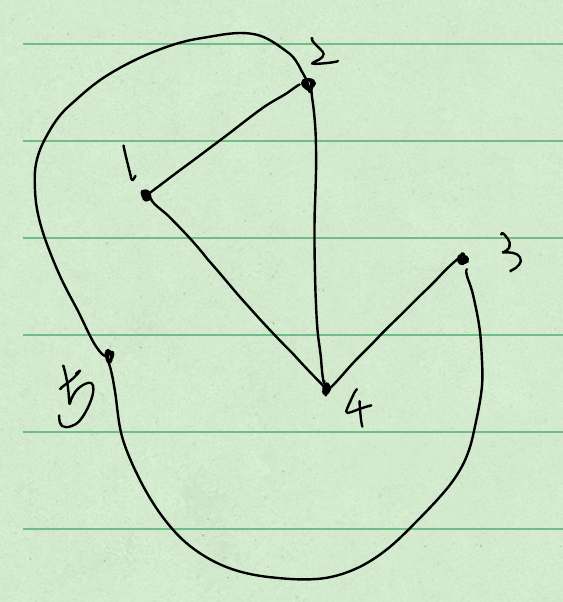
\includegraphics[width=0.2\textwidth]{graph.png}}

\subsection{Two representation of Graph}
When we talk about graph without adjective, that means it is a 
undirected graph. Suppose the number of vertices is $|V| = n$.
\begin{itemize}
 \item A vertex is incident to an edge if the vertex is one of the two vertices 
the edge connects.
\item If an edge $(u, v)$ has end points $u$ and $v$, we say it is an incident 
to vertex $u$ and $v$.
\item $u$, $v$ are adjacent if $(u, v) \in \mathbb{E}$.
\item The degree of vertex $v$ is the number of edges incident on $v$.
\end{itemize}

\subsubsection{Adjacency Matrix}
Adjacency Matrix is an symmetric matrix for undirected graph where
\[
V_{ij} = 
\begin{cases*}
 |(i,j)| & ,\text{ if $(i,j) \in \mathbb{E}$.}\\
 0  &,\text{ otherwise.}
\end{cases*}
\]

Space = $O(n^2)$.
\subsubsection{Adjacency List}
Adjacency List is an array of size $n$ of linked list, where $i$-th entry is 
a linked list consisting of the neighbors of vertex-$i$. It is default  representation of graph.

Space = $O(n + m)$.
\newpage
\subsection{Connectivity}
\subsubsection{Path}
A path in a graph is a sequence of vertices
\[v_0 v_1 \cdots v_k\]
, such that $(v_i, v_{i+1}) \in \mathbb{E}$ for $i = 0, 1, 2, \cdots, k-1$.

A simple path is a path that does not repeat vertices.
\paragraph{Lemma:}
If there is a path $(u, v)$, there must be a simple path $(u, v)$.
\subsubsection{Cycle}
A cycle in a graph is a sequence of vertices
\[v_0 v_1 \cdots v_kv_0\]
, such that $(v_i, v_{i+1}) \in \mathbb{E}$ for $i = 0, 1, 2, \cdots, k-1$ and 
$(v_k, v_{0}) \in \mathbb{E}$. All $v_i$'s are distinct.

\subsubsection{Connectivity}
\begin{itemize}
 \item $u$, $v$ is \textbf{connected} if there is a path between them.
 \item $G$ is \textbf{connected} if $\forall u, v \in V$, there is a path 
between $u$ and $v$.
\item The \textbf{connected components} of $G$ are maximal subset of vertices 
that are pairwise connected.
\end{itemize}

\subsubsection{Connection is equivalence relation}
Connection relation in a graph is an equivalence relation.
\begin{itemize}
 \item Reflexive Relation (take Path of length 0)
 \item Symmetric Relation (reversible path)
 \item Transitive Relation: If a Graph has a $uv$ path and also $vw$ path then 
it will also contain $uw$ path.
\end{itemize}
Because connection is the equivalence relation, pairwise connected vertices 
form a connected component.